\documentclass{article}
\usepackage[a4paper,margin=1.6cm]{geometry}
\usepackage{tikz}
\usetikzlibrary{positioning,arrows.meta,shapes.geometric}

\begin{document}

\begin{figure}[htbp]
\centering
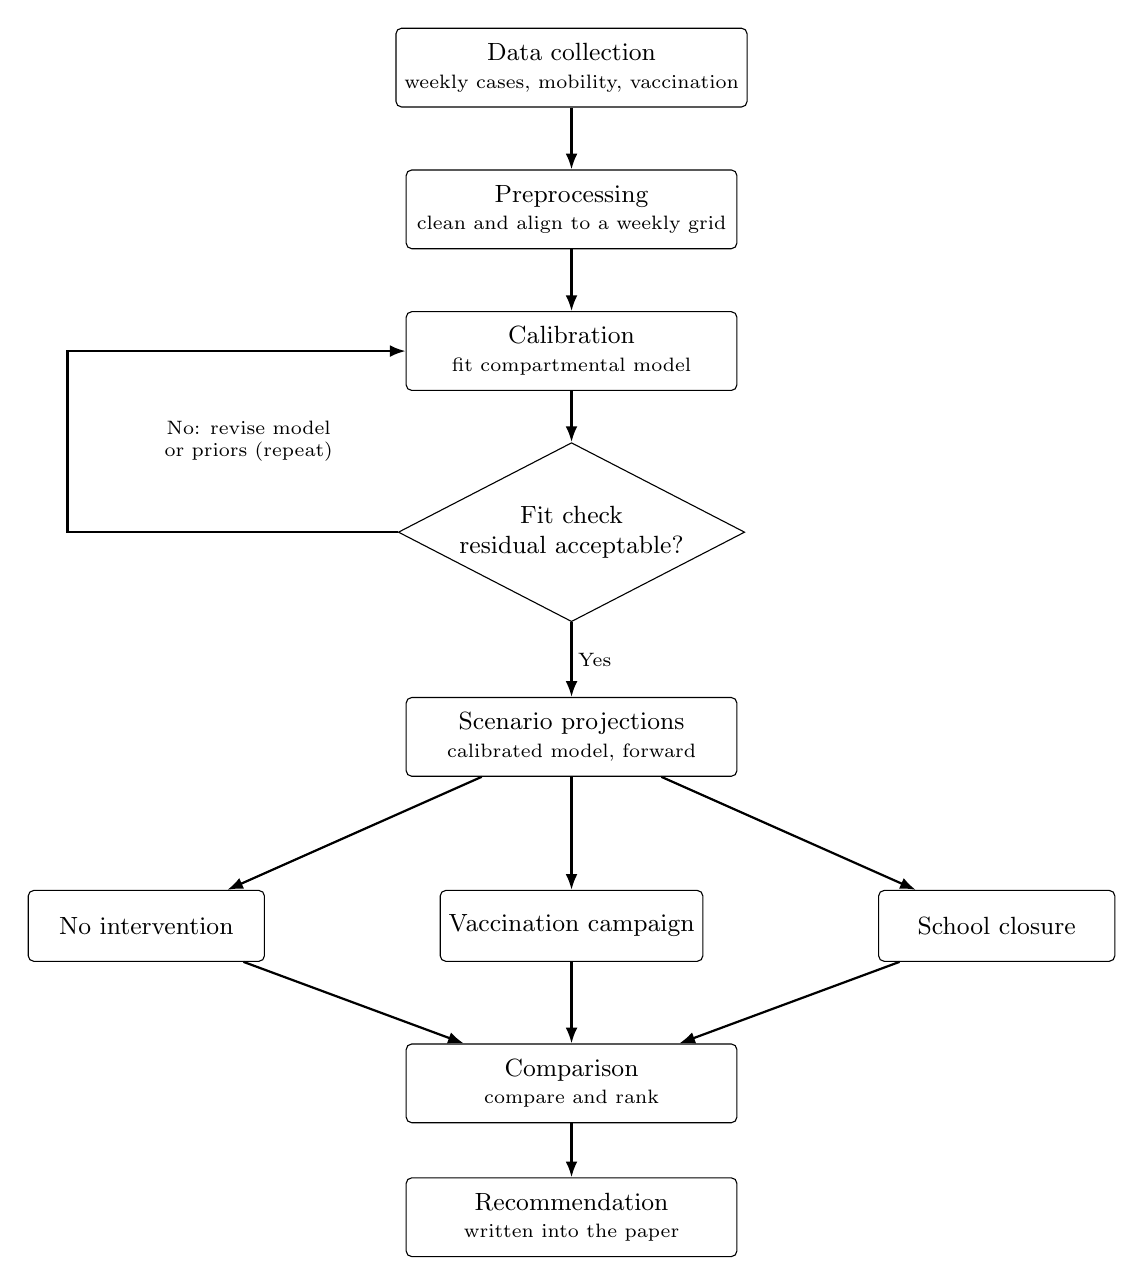
\begin{tikzpicture}[
  font=\small,
  box/.style={draw, rounded corners=2pt, align=center,
              minimum width=42mm, minimum height=10mm, inner sep=3pt},
  pol/.style={draw, rounded corners=2pt, align=center,
              minimum width=30mm, minimum height=9mm, inner sep=3pt},
  decision/.style={draw, diamond, aspect=1.9, align=center,
                   inner sep=1pt, minimum width=44mm, minimum height=16mm},
  arr/.style={-{Latex[length=2mm]}, thick},
  lbl/.style={font=\scriptsize, inner sep=2pt, align=center},
]

% ---- main spine -------------------------------------------------
\node[box] (data)  at (0,0)      {Data collection\\[-1pt]{\scriptsize weekly cases, mobility, vaccination}};
\node[box] (prep)  at (0,-1.8)   {Preprocessing\\[-1pt]{\scriptsize clean and align to a weekly grid}};
\node[box] (calib) at (0,-3.6)   {Calibration\\[-1pt]{\scriptsize fit compartmental model}};
\node[decision] (check) at (0,-5.9) {Fit check\\ residual acceptable?};
\node[box] (proj)  at (0,-8.5)   {Scenario projections\\[-1pt]{\scriptsize calibrated model, forward}};
\node[pol] (p1) at (-5.4,-10.9)  {No intervention};
\node[pol] (p2) at (0,-10.9)     {Vaccination campaign};
\node[pol] (p3) at (5.4,-10.9)   {School closure};
\node[box] (comp)  at (0,-12.9)  {Comparison\\[-1pt]{\scriptsize compare and rank}};
\node[box] (rec)   at (0,-14.6)  {Recommendation\\[-1pt]{\scriptsize written into the paper}};

% ---- spine arrows -----------------------------------------------
\draw[arr] (data)  -- (prep);
\draw[arr] (prep)  -- (calib);
\draw[arr] (calib) -- (check);
\draw[arr] (check) -- (proj) node[midway, right, lbl] {Yes};
\draw[arr] (proj)  -- (p1);
\draw[arr] (proj)  -- (p2);
\draw[arr] (proj)  -- (p3);
\draw[arr] (p1)    -- (comp);
\draw[arr] (p2)    -- (comp);
\draw[arr] (p3)    -- (comp);
\draw[arr] (comp)  -- (rec);

% ---- revise-and-return loop -------------------------------------
\draw[arr] (check.west) -- (-6.4,-5.9) -- (-6.4,-3.6) -- (calib.west);
\node[lbl] at (-4.1,-4.75) {No: revise model\\or priors (repeat)};

\end{tikzpicture}
\caption{Schematic of the epidemic-control modelling workflow. Weekly case counts,
mobility traces and vaccination coverage are assembled for the study city and, in
preprocessing, cleaned and aligned onto a common weekly grid. Transmission
parameters are estimated by fitting a compartmental model to the aligned data
(calibration); if the fit residual is unacceptable the model structure or the
priors are revised and calibration is repeated, and once the fit is accepted the
calibrated model is projected forward under three policies (no intervention, a
vaccination campaign, and school closure). The three projections are compared and
ranked, and the ranking is written up as the paper's recommendation.}
\end{figure}

\end{document}
